\section{轮建模分析}
\subsection{实体建模方案}
\subsubsection{方案一}
根据制作图\ref{fig:xiaoluntaotong}所示套筒三维模型的经验,可以将图\ref{fig:xiaolunlun.pdf}所示的轮零件拆分为图\ref{fig:lunfenxi1.png}所示的套筒和\ref{fig:lunfenxi2.png}所示结构的组合。\ref{fig:lunfenxi2.png}所示结构又可以以此方式进一步简单为两个套筒的组合。这种简化方案的三维建模过程简单,难点主要在于各个组成部分的定位,需要利用套筒模型的轴心线的中点进行定位,才能够获得准确的模型。故需要绘制轴心辅助线,以利于组合定位。
\begin{figure}[htbp]
\centering
\subfloat[]{\label{fig:lunfenxi1.png}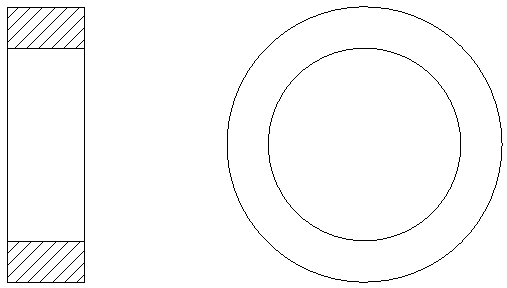
\includegraphics[scale=0.4]{lunfenxi1.png}}\hspace{20pt}
\subfloat[]{\label{fig:lunfenxi2.png}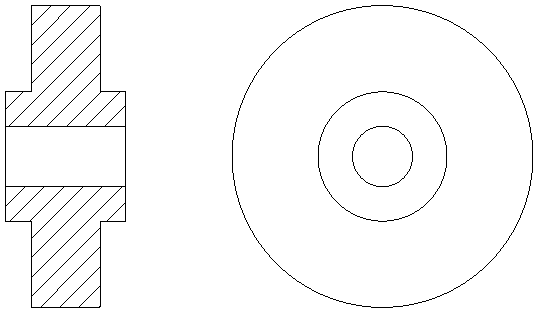
\includegraphics[scale=0.25]{lunfenxi2.png}}
\caption{轮实体建模方案一}
\end{figure}
\subsubsection{方案二}

注意到图\ref{fig:xiaolunlun.pdf}中的主视图不仅具有上下对称的特点,同时还具备上下对称的特性。故可以先构一半的模型,然后利用镜像来快速构建另一半模型。因此,图\ref{fig:xiaolunlun.pdf}所示的轮零件可以图\ref{fig:lunfenxi3.png}所示$\frac{1}{2}$长的套筒,然后减去图\ref{fig:lunfenxi4.png}所示的套筒,来获得图\ref{fig:lunfenxi5.png}所示模型,最后,利用镜像构建另一半模型。这种建模方案定位比较方便,不需要绘制用于定位的辅助线,构建方式也简单直接。
\begin{figure}[htbp]
\centering
\subfloat[]{\label{fig:lunfenxi3.png}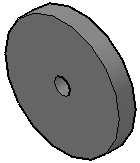
\includegraphics[scale=0.6]{lunfenxi3.png}}\hspace{20pt}
\subfloat[]{\label{fig:lunfenxi4.png}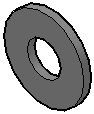
\includegraphics[scale=0.6]{lunfenxi4.png}}\hspace{20pt}
\subfloat[]{\label{fig:lunfenxi5.png}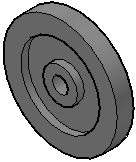
\includegraphics[scale=0.6]{lunfenxi5.png}}
\caption{轮实体建模方案二}
\end{figure}

当然,还存在其它的实体建模方案,这里就不一一赘述。读者有兴趣,可以逐尝用多种不同的构建方案进行三维模型构建,仔细体会每种组合方式的特点。
\subsection{旋转建模方案}

\begin{figure}[htbp]
\centering
\subfloat[]{\label{fig:lunfenxi6.png}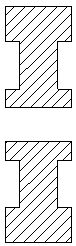
\includegraphics[scale=0.7]{lunfenxi6.png}}\hspace{40pt}
\subfloat[]{\label{fig:lunfenxi7.png}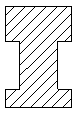
\includegraphics[scale=1]{lunfenxi7.png}}
\caption{轴旋转建模方案}
\end{figure}

基于图\ref{fig:xiaolunlianjiegan}所示连接杆的三维建模经验,图\ref{fig:xiaolunlun.pdf}所示的轮零件忽略圆角后具有图\ref{fig:lunfenxi6.png}所示的截面,因此可绘制图\ref{fig:lunfenxi7.png}所示的轮廓线来构成旋转特征面,并通过旋转的方式来完成模型的构建。这种建模方式也比较简单快捷。

\yaodian{尝用不同的方式构建模型,能有效提升灵活解决问题的能力。}
\endinput